\documentclass[12pt,a4paper]{article}

% 如果需要中文支持,推荐使用xeCJK + 字体设置
\usepackage{xeCJK}
\setCJKmainfont{SimSun}  % 示例:宋体,可根据系统字体情况更换
\usepackage{amsmath}      % 数学公式(如有需要)
\usepackage{graphicx}     % 插图
\usepackage{geometry}     % 调整页边距
\usepackage{fancyhdr}     % 自定义页眉页脚
\usepackage{indentfirst}  % 中文首行缩进
\usepackage{calc}         % 允许做长度运算(测量文字宽度等)
\usepackage{titlesec}
\usepackage{booktabs} % 解决 \midrule 和 \bottomrule 报错
\usepackage{enumitem} % 支持自定义列表格式
\usepackage{float}
\usepackage{subcaption}
\usepackage{tabularx}
\usepackage{float}

% 设置 \section 级标题为:加粗、大字号(如 \Large)
\titleformat{\section}
	{\bfseries\large}    % 标题自身的格式
	{\thesection}        % 标题编号的显示方式
	{1em}                % 编号与标题文字之间的间距
	{}                   % 在标题文字前后可插入额外代码,此处为空
	
% 设置 \subsection 级标题为:加粗、中等字号(如 \normalsize)
\titleformat{\subsection}
	{\bfseries\normalsize}
	{\thesubsection}
	{1em}
{}

% 页面设置(可根据需要微调)
\geometry{
	left=2cm,
	right=2cm,
	top=1cm,
	bottom=1.5cm
}

% 不需要过大的行距,使用较接近单倍行距的设置
\renewcommand{\baselinestretch}{1}

% 仅在页脚居中显示页码,页眉保持为空
\pagestyle{fancy}
\fancyhf{}  % 清空默认的页眉页脚
\fancyfoot[C]{\thepage}
\renewcommand{\headrulewidth}{0pt}
\renewcommand{\footrulewidth}{0pt}

% 首行缩进2字符(中文习惯)
\setlength{\parindent}{0pt}
\setlength{\leftskip}{2em}

\begin{document}
	%-------------------------------------------------------
	% 1 并排两个minipage:左标题、右校徽
	%   - 0.65\textwidth + 0.35\textwidth = \textwidth
	%   - 如果校徽过大或过小,可改宽度,如 0.25\textwidth、0.3\textwidth 等
	%   - 如果想让标题更大,可将 \Huge 改成 \huge 或 \LARGE
	%-------------------------------------------------------
	\noindent
	\hspace{-2em}
	\begin{minipage}[c]{0.65\textwidth}
		\raggedright
		{\fontsize{40pt}{60pt}\selectfont 物理实验报告}
	\end{minipage}
	\begin{minipage}[c]{0.35\textwidth}
		\raggedleft
		% 强制把校徽拉大到 0.35\textwidth 宽度 (高度自动匹配)
		% 若想指定高度,可用 "height=3cm" 等. 二选一即可.
		
\includegraphics[width=\linewidth, trim={20cm 20cm 20cm 20cm}, clip]{university_logo.png}
	\end{minipage}

	\vspace{-1em}
	

	%下方画两条分割线,并在两线之间写学号、姓名、日期、时间
	
	\hrule
	\vspace{0.4em}
	\noindent
	\begin{tabular}{l l l l}
    学号:\underline{114514} & 姓名:\underline{SUSTech} &
    日期:\underline{2025/04/15} & 时间:\underline{周二下午}
	\end{tabular}
	\vspace{-0em}
	\par
	\hrule

	

	%正文示例

	
	\section{实验名称:线性与非线性元件伏安特性的测量}
	
	\section{实验目的}
	\begin{enumerate}
		\item 熟练使用电学实验的常用仪器,掌握电流、电压、电阻等电学量的测量方法。
		\item 理解制流电路和分压电路的工作原理,学习恒压源与恒流源的使用。
		\item 测量小灯泡的伏安特性曲线,掌握电流表的内接法和外接法。
		\item 测量发光二极管及稳压二极管的伏安特性曲线。
	\end{enumerate}

	\section{实验原理}
	1、制流电路、分压电路、电流表内接法、电流表外接法
		\begin{figure}[H]
		\centering
		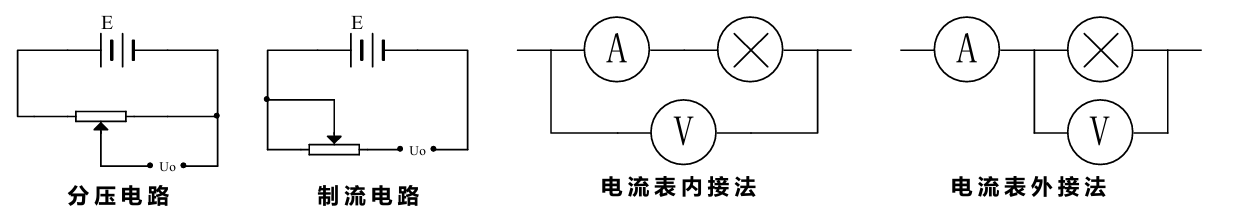
\includegraphics[width=1\textwidth]{电路图.png} % 这里替换为你的 PNG 文件名
		\caption{电路图}
		\label{fig:example}
	  	\end{figure}
	2、恒压源、恒流源\\
	恒压源就是常说的稳压电源,在额定输出电流范围内,能够对负载提供稳定的输出电压。理想的恒压源内阻为零,负载改变时,输出电流发生相应变化,输出电压维持恒定不变;\\
	恒流源也叫稳流电源,在额定输出电压范围内,能够对负载提供稳定的输出电流。理想的恒流源内阻为无穷大,负载改变时,输出电压发生相应变化,输出电流维持恒定不变。\\
	更高级的电源由恒压和恒流两部分组成,两种工作状态自动切换。电源工作在恒压状态时,恒流部分起限流保护作用;电源工作在恒流状态时,恒压部分起限压保护作用。
	
	\section{实验仪器}
	稳压电源,稳流电源,毫安表,万用表,小灯泡,发光二极管,稳压二极管,导线若干

	\section{实验内容}
		\subsection{测量钨丝小灯泡和定值电阻的伏安特性曲线}
			\begin{enumerate}[label=\arabic*.]
			\item 分别采用电流表内接法和电流表外接法测量小灯泡的伏安特性曲线。使用恒压电源输出,逐渐增大电压,记录对应的电流值。要求电压在 \(0\sim7.000\,\text{V}\) 范围内,每隔 \(\sim0.500\,\text{V}\) 记录一组数据点。
			\item 根据(1)中所测数据,在同一坐标系中绘制两条小灯泡的伏安特性曲线(\(V\text{--}I\) 曲线),比较内接法伏安特性曲线和外接法伏安特性曲线的差异,定性分析差异产生的原因。
		\end{enumerate}

		\subsection{测量发光二极管的伏安特性曲线}
			\begin{figure}[htbp]
				\centering
				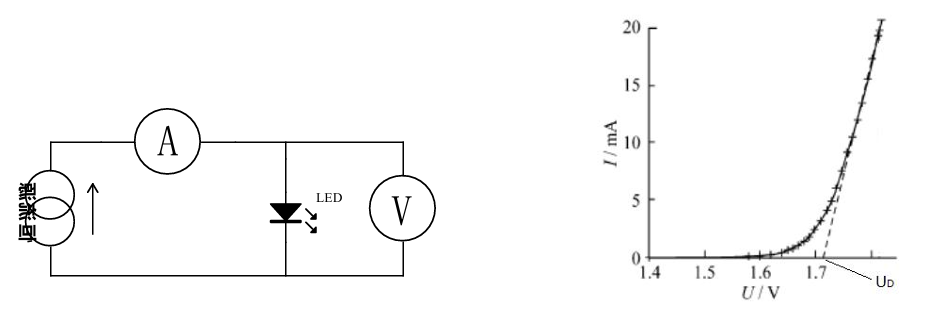
\includegraphics[width=0.6\textwidth]{发光二极管.png} % 这里替换为你的 PNG 文件名
				\caption{发光二极管伏安特性曲线}
				\label{fig:example}
	  		\end{figure}
			\begin{enumerate}[label=\arabic*]
				\item 使用恒流源,按照电流表外接法电路图连接电路。
				\item 逐渐增大电流,记录相应的电压值,分别测量红色、绿色、蓝色发光二极管的正向伏安特性曲线。
				\item 根据(2)中所测数据,在同一坐标系中绘制三种发光二极管的正向伏安特性曲线。
				\item 根据发光二极管的正向伏安特性曲线,得到发光二极管的阈值电压 \(U_D\),并根据下面的公式$eU_\mathrm{D}{=}h\frac{c}{\lambda}$计算三种发光二极管的发光波长 \(\lambda\)。
			\end{enumerate}

		\subsection{测量稳压二极管的伏安特性曲线}
		参考发光二极管伏安特性曲线的测量方法,自拟表格,分别测量稳压二极管的正向和反向伏安特性曲线。为了避免二极管烧坏,确保正反向电流均不超过50mA。根据所测数据,在同一坐标系中绘制稳压二极管的正向和反向伏安特性曲线。
			\begin{figure}[htbp]
				\centering
				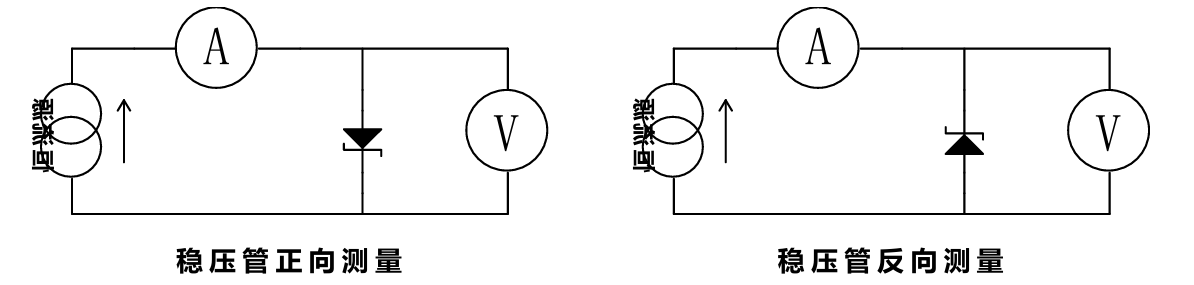
\includegraphics[width=0.6\textwidth]{稳压二极管.png} % 这里替换为你的 PNG 文件名
				\caption{稳压二极管伏安特性曲线}
				\label{fig:example}
		  	\end{figure}

	\section{数据记录}
		进行实验,记录数据,并输入进excel
		\begin{figure}[htbp]
			\centering
			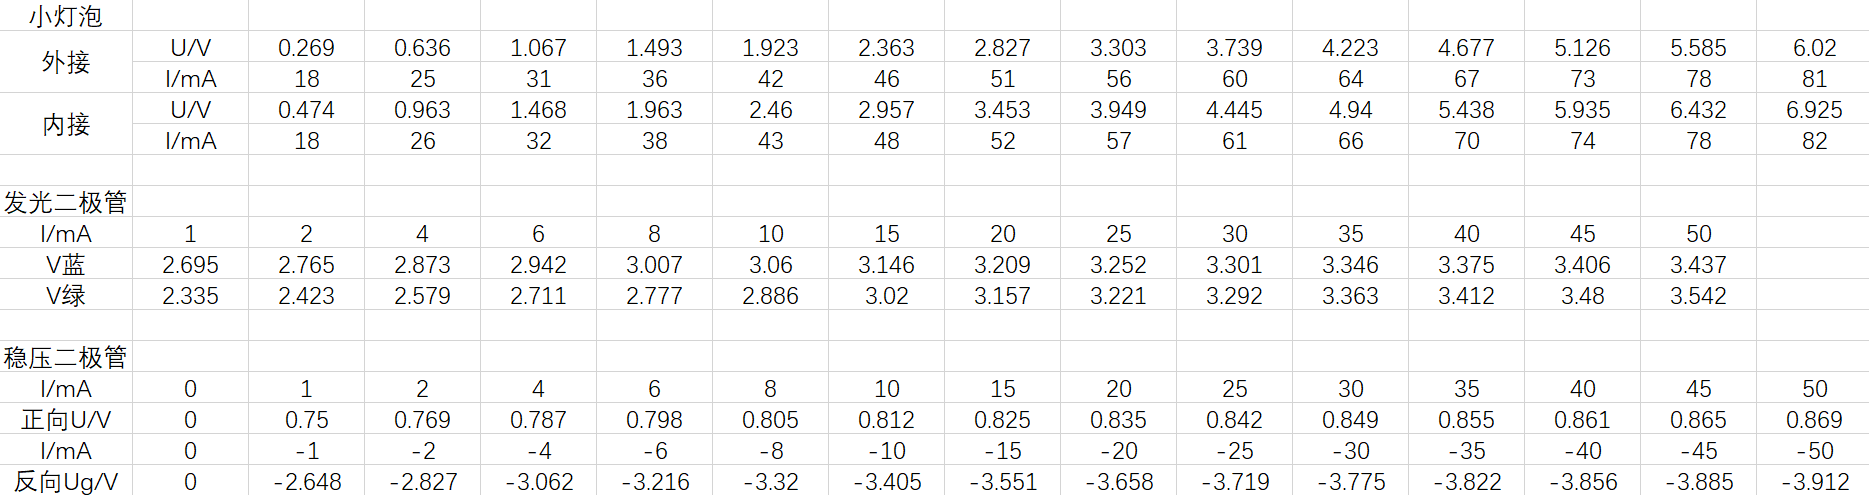
\includegraphics[width=1\textwidth]{数据处理.png} % 这里替换为你的 PNG 文件名
			\caption{实验数据}
			\label{fig:example}
		  \end{figure}

	\section{数据处理}
		\subsection{钨丝小灯泡和定值电阻的伏安特性曲线}
			由实验数据作出钨丝小灯泡和定值电阻的伏安特性曲线,并进行分析
			\begin{figure}[H]
				\centering
					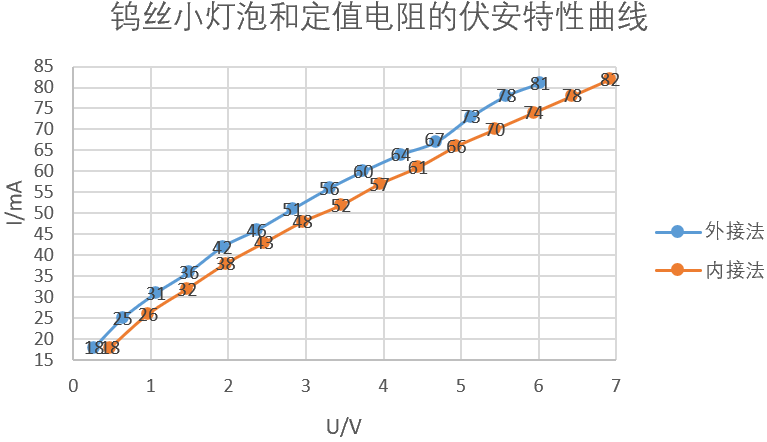
\includegraphics[width=0.5\textwidth]{小灯泡.png} % 这里替换为你的 PNG 文件名
				\caption{钨丝小灯泡和定值电阻的伏安特性曲线}
				\label{fig:example}
		  	\end{figure}
			由曲线可知:
			\paragraph{V相同时$I_{\text{内}}<I_{\text{外}}$\\}
				分析:由于$I_{\text{内}}=\dfrac{V}{R_{\text{灯}}+R_A},\;I_{\text{外}}=\dfrac{V}{R_{\text{灯}}}+\dfrac{V}{R_V}$。又有$R_{\text{灯}}^2+R_{\text{灯}}R_A+R_AR_V>0 \implies (R_{\text{灯}}+R_V)(R_{\text{灯}}+R_A)>R_{\text{灯}}R_V \implies \dfrac{1}{R_{\text{灯}}+R_A}<\dfrac{1}{R_{\text{灯}}}+\dfrac{1}{R_V} \implies \dfrac{V}{R_{\text{灯}}+R_A}<\dfrac{V}{R_{\text{灯}}}+\dfrac{V}{R_V} \implies I_{\text{内}}<I_{\text{外}}$。
			\paragraph{误差\\}
				内接法的伏安特性曲线整体位于外接曲线的左上方。内接法的误差来源:电流表分压,$\Delta V = I \cdot R_A$,误差随电流增大线性增加,导致小灯泡的等效电阻计算值偏大,$R_{\text{测}} = R_L + R_A$。\\
				外接法的误差来源:电压表分流,$\Delta I = \dfrac{V}{R_V}$,误差随电压增大线性增加,导致等效电阻计算值偏小,$R_{\text{测}} = \dfrac{R_L R_V}{R_L + R_V}$。
		
		\subsection{发光二极管的伏安特性曲线}
			由实验数据作出发光二极管的伏安特性曲线,并进行分析
			\begin{figure}[H]
				\centering
					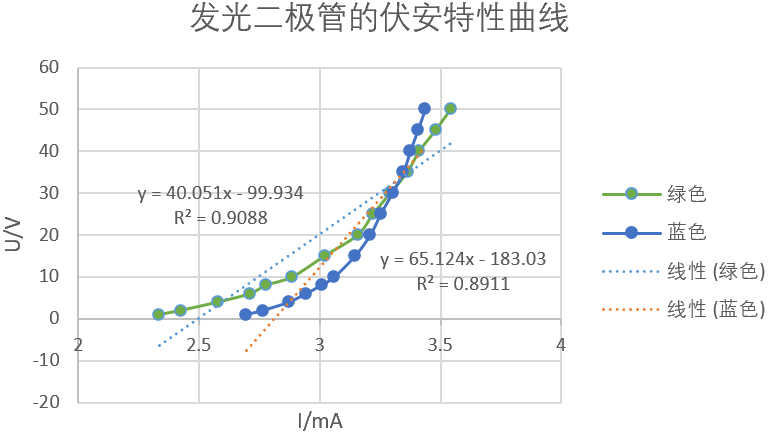
\includegraphics[width=0.5\textwidth]{发光.png} % 这里替换为你的 PNG 文件名
				\caption{发光二极管的伏安特性曲线}
				\label{fig:example}
		  	\end{figure}
			对两条曲线最后五组数据进行线性拟合,得到x轴截距,即两种发光二极管的阈值电压分别为$U_G \approx 2.91\,V,\;U_B \approx 3.11\,V$。由公式$eU_D=h\dfrac{c}{\lambda}$,即$\lambda=\dfrac{hc}{eU_D}$,得到两种发光二极管的波长分别为:
			$$\lambda_G=\dfrac{6.626\times10^{-34}\,J\cdot s \times 2.998\times10^8\,m\cdot s^{-1}}{1.602\times10^{-19}\,C\times2.91\,V} \approx 426.1\,nm$$
    		$$\lambda_B=\dfrac{6.626\times10^{-34}\,J\cdot s \times 2.998\times10^8\,m\cdot s^{-1}}{1.602\times10^{-19}\,C\times3.11\,V} \approx 398.7\,nm$$
    
		\subsection{稳压二极管的伏安特性曲线}
			根据实验数据做出稳压二极管的伏安特性曲线:
			\begin{figure}[H]
				\centering
				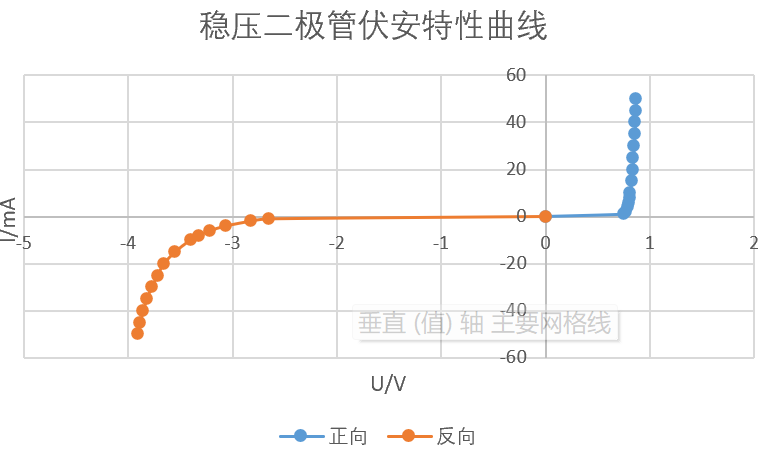
\includegraphics[width=0.4\textwidth]{稳压.png} % 这里替换为你的 PNG 文件名
				\caption{稳压二极管的伏安特性曲线}
				\label{fig:example}
		  	\end{figure}
			

	\section{误差分析}
		1.实验仪器精度不足;\qquad	2.导线有电阻;\qquad 3.发光二极管的光不是单色光,有杂光; 
		4.电流的热效应导致元件升温而电阻发生变化。



	\section{问题思考}
		探讨两种颜色发光二极管伏安特性曲线的相似与不同之处,并给出合理的解释。\\
		相似之处: 随着电压增大,伏安曲线先缓慢上升,之后迅速爬升,且在较高电压下呈现出近似线性的增长趋势。\\
		解释:当正向电压较小时,二极管处于截止状态,PN 结的内建电场尚未被完全中和,载流子扩散受限,故电流随电压变化较小,使曲线呈现平缓上升;当电压超过开启电压后,二极管进入导通状态,载流子大量注入,电流迅速增大,曲线斜率急剧上升,呈指数增长趋势;继续增大电压时,由于电流主要受外部限流电阻控制,曲线整体上趋向于线性增长。\\
		不同之处: 导通状态下,两种颜色发光二极管伏安曲线中线性部分延长线与 x 轴的交点(即阈值电压)存在差异。\\
		解释: 不同颜色的发光二极管采用的半导体材料不同,导致 PN 结特性存在差异。波长较短的发光二极管(如蓝色)需要更高能量以促使电子与空穴复合释放光子,因此其阈值电压较高;而波长较长的发光二极管(如红色)的阈值电压则相对较低。
	
	\section{实验结论}
	本次实验测量并绘制了钨丝小灯泡、绿色和蓝色发光二极管、稳压二极管正反向的伏安特性曲线。通过计算得到两种发光二极管发出光的波长分别为$\lambda_G=426.1\,nm,\;\lambda_B=398,7\,nm$。
\end{document}
